\documentclass[pdftex,12pt,letter]{article}
\usepackage[margin=0.75in]{geometry}
\usepackage{verbatim}
\usepackage{graphicx}
\usepackage{xspace}
\usepackage{cite}
\usepackage{url}
\usepackage[pdftex,pdfpagelabels,bookmarks,hyperindex,hyperfigures]{hyperref}

\newcommand{\pd}{protoDUNE\xspace}
%\newcommand{\pdsp}{pD/SP\xspace}
\newcommand{\xrd}{XRootD\xspace}
\newcommand{\expname}{\textit{NP04}\xspace}

\title{Technical Proposal for Prompt Processing System in the Single-Phase \pd}
\date{\today}
\author{M.\,Potekhin and B.\,Viren}


\begin{document}
\maketitle

\begin{abstract}
\noindent  This note describes a proposal for the design of
the prompt processing system in the Single-Phase \pd
(CERN experiment \expname). We start with a brief summary of the data characteristics and data handling patterns
as documented in DocDB\,1086 \cite{docdb1086}, DocDB\,1212 \cite{docdb1212} and present a design which
satisfies the basic requirements set forth in  DocDB 1811 \cite{docdb1811}.
\end{abstract}

%%%%%%%%%%%%%
\section{Overview}
\subsection{Data Scenarios and Data Handling}
\label{sec:rawdata}
Quantitative information about scenarios for data taking in \pd is collected and maintained in \cite{docdb1086}. The following parameters
are assumed at the time of writing: the raw data rate will 1.4\,GB/s after lossless compression, and to size up
the system and account for contingencies rates up to 3\,GB/s are under consideration.

Outline of the design of the raw data handling system is documented in  \cite{docdb1212} and other prior \pd documentation.
According to it, the data is tranmitted from the online buffer to the CERN EOS via a 20 Gbps full-duplex network connection.
The EOS system serves as the hub and staging area for the \pd raw data from which
it gets committed to the tape archive at CERN and also transmitted to FNAL and potentially
other US and international locations. All or most links in the data transmission chain will be based on F-FTS.

\subsection{Outline of Prompt Processing}
\label{sec:outline}
According to \cite{docdb1811}  prompt processing needs to occur on the scale
of tens of minutes (or better) from the time the data was taken. It's purpose is to
provide a more in-depth data QA and assessment of the detector operating conditions
than is afforded by most basic histogramming e.g. of the ADC counts. Most calculations
done as a part of prompt processing will result in some sort of a ``visual product'', i.e. a histogram,
plot, event display or a summary table in order to provide optimal accessibility to the experiment
operators.


\subsection{Scope of the Prompt Processing}
This is a compressed summary of information presented in \cite{docdb1811}.
For more detailed explanation please see the source.

\subsubsection{Data Processing}
\label{sec:categories}
The categories are as follows:

\begin{description}

\item[DAQ] A summary of DAQ-level data (with no decompression) such as summaries of data
 rates  or summaries of any metadata, status codes the provided by the DAQ etc.
This processing is a candidate for running directly within artDAQ
monitor processes instead of prompt-processing and is included here
for completeness.

\item[ADC] A summary of ADC-level data e.g. mean/RMS (requires data decompression).


\item[FFT] A summary of the ADC-level data in frequency space. It requires running a discrete Fourier
transform (FFT) on channel waveforms. This largely  provides measures of noise and its
evolution.

\item[Sig] A summary of the data \textit{after signal processing}.
The processing is in  frequency space and so uses the output of FFT.  It includes software
noise subtraction, filtering and deconvolution of the response function.

\item[Reco] Results from running some type of reconstruction (perhaps simplified).
It may, for  example, provide a coarse count of straight muon track candidates.

\end{description}


\noindent It is possible that \textbf{ADC} and \textbf{FFT} stages will be implemented as a single processing
block since \textbf{FFT} will require uncompressed data in any case.

\subsubsection{Downsampling}
\label{sec:downsampling}
The categories of processing as outlined above may have drastically different resource requirements.
%i.e. the ability to select a fractional sample of the data stream as is progresses through the chain, at every stage.
For example, if 100 cores are allocated to FFT calculation this may be done for approximately 10\% of the events
in streaming mode. Then, depending on the type of deconvolution being employed (1D vs 2D) this step
may require an order of magnitude more CPU to complete. To stay within reasonable footprint,
it may be necessary to put only a fraction of the output of the FFT stage through deconvolution stage
(note that the FFT output is valuable in and by itself). Event reconstruction will in turn require even more CPU
and so it may also be necessary to scale down the number of
events at this stage (while still aiming for quick turnaround). So effectively we are considering ``downsampling''
of data as it progresses in the prompt processing chain.



\subsubsection{Visualization}
The \textit{Visualization} category of processing
 may take data output from any of the above listed stages in
order to efficiently present it to the end-user. 
% This stage will need to
%have a sampling fraction  based on both the processing requirements
%(e.g. processing time) and based on how fast a human can absorb and understand
%the information as it undergoes updates.
It may include items such as:

\begin{itemize}

\item Histograms of statistical quantities.

\item Strip charts showing their history.

\item Various statistics dynamically updated over some some fixed time window.

\item 2D displays of underlying values such as spectrograms of the \textit{FFT}
  output (vs wire), or time vs wire using output from \textit{ADC} and \textit{Sig}.

\end{itemize}

\subsubsection{Other Applications of the Data Processing Components}
Results of the intermediate stages of Data Processing may need to be preserved, for
example the data in graphic form for audit/run documentation purposes.
Also, there could be a potential for large processing efficiency
gains to be made if the entire data can be run through the \textit{Sig} processing followed by ZS.


\subsection{Prompt Processing as a DAG}
\label{sec:dag}
Data and processes involved in prompt processing as outlined in \ref{sec:outline} can be
modeled together as a DAG.An example of such a model is given in Fig.\ref{fig:dag1}.

\begin{figure}[tbh]
  \centering
  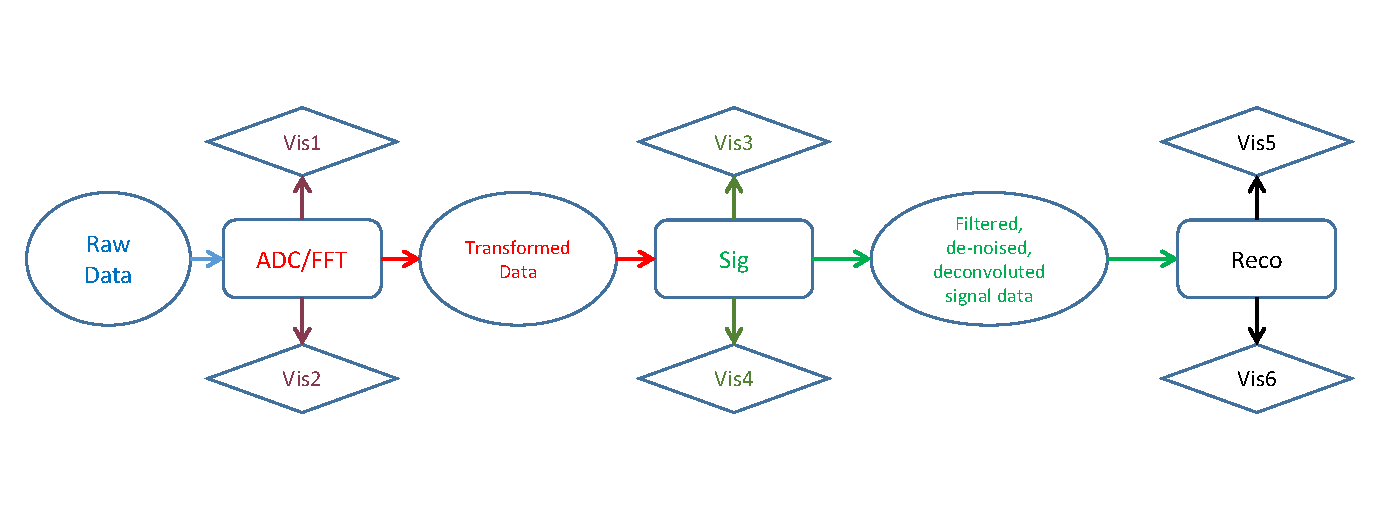
\includegraphics[width=1.0\textwidth]{figures/prompt_dag_1.pdf}
  \caption{An example of DAG representing prompt processing in \expname.}
  \label{fig:dag1}
\end{figure}
\section{Design Parameters}
\subsection{Staging Data for Prompt Processing}
CERN EOS appears to be the best suited platform from which to
serve the data for prompt processing for the following reasons:
\begin{itemize}

\item The online buffer is likely to operate at a significant data rate (see above) and additional I/O load on the buffer is undesirable
due to practical limits on the storage bandwidth and in order to guarantee stability of operation for the online buffer and DAQ in general.

\item It can be be expected that the data arrives to EOS rather quickly after having been captured in the online buffer (e.g.$\sim$1\,min) so
the latency due to this transfer is acceptable.

\item EOS has variety of interfaces including \xrd which simplifies access from various types of locations (both inside and outside the CERN perimeter).
Leveraging this capability of EOS will allow to avoid implementaion of a special data transmission handling chain for prompt processing (such as explicit
file copy to the Worker Node and back).


\end{itemize}

\subsection{Prioritization of Processing Steps}
Quick turnaround is the key for the prompt processing to be useful. For each processing category
to be complete it must include the visualization component in order to make the results available
to the experts. What fraction of the total stream of events ends up being processed is relatvely less
important compared to timely completion of all steps (NB. with downsampling of the data, see 
\ref{sec:downsampling}).

A use case may help to illustrate this. Let's assume a predetermined fraction of the events needs to
be reconstructed (perhaps with simplified algorithm aimed at identifying cosmic muon candidates).
This information needs to be made available to the operators as quickly as possbile in order to ascertain the performance
of the detector at a level of confidence much higher than that provided by ADC histograms.
Consider the case where the \textbf{FFT} and \textbf{Sig} parts (see \ref{sec:categories})
completed satisfactorily but are consuming a fraction of the computing resource so large that
the  \textbf{Reco} stage is starved of resources and takes a very long time to complete, making
it less relevant and less useful. This situation can be prevented by prioritizing each step higher
than the preceding one (again, with downsampling as per \ref{sec:downsampling}).

It is therefore necessary to provide a mechanism for flexible prioritization of the different
classes of jobs running in the prompt processing system.



\subsection{Workflow: Automation And State}

Prompt processing represents a use case quite different from managed production or user analysis, and is closer to
procesing data in streaming mode. It is rather obvious that manual job submission won't scale to the needs
of the experiment, and it will be necessary to automate the prompt processing workflow.

Automation can be achieved in  number of different ways. In the simples case, processes belonging to a particular stage of processing
can be waiting for files produced by the previous
stage and matching a particular name pattern (in a fashion similar to the ``dropbox'' mechanism). In this case it is the file
system which keeps the state of the workflow. Consider jobs performing calculations in the \textbf{Sig} stage that are waiting for
files containing the output of the \textbf{FFT} stage.
These scheme is conceptually simple but has a number of disadvantages, such as
\begin{itemize}
\item Matching multiple jobs to multiple files is not trivial and there may be race conditions etc
\item Detection of error status would require additional scripting
\item Likewise, generating a view of workload distribution across the processing stages is possible but requires
scripting
\item Changing characteristics of the workload is complicated
\item Bookkeeping is difficult
\end{itemize}

\noindent Problems listed above can be alleviated if the state of the workflow is kept in a database.

\subsection{Resource Utilization}
The system is required to be flexible enough to take advantage of varying type of resources. For example, the ``neut'' cluster at CERN
is a rather vanilla example of a HTCondor installation. It will be scaled to up to 350 nodes with multiple cores each. It does not have Grid middleware
installed and technically this should not be necessary since it's local to the data. This implies that it must be possible to generate jobs to
run on this cluster locally.

Flexibility needs to be retained to utilize the lxbatch facility at CERN or even run jobs on the facilities at FNAL, BNL and other such locations
in the US and Europe. This is possible by utilizing EOS interfaces such as XRootD.

As mentioned above, it may be required to explore computing resources
at other institutions.  Such explorations must consider the nominal
turn around time that makes this processing ``prompt''.

\subsection{Monitoring}
It will be neccesary to monitor the prompt processing system at a few
levels, from general availability and throughput of the computing
element to individual job level and log file information.  A web
service will be required to ensure optimal and user-friendly interface
to the monitoring system.

Another web service (potentially integrated with the above) is
required to display results of the \textit{Vis} stage for use by
detector experts, commissioning and operations shift workers as well
as general collaborators who may not be at CERN.  Some requirements
for this web service(s) are:

\begin{itemize}
\item Display current and past sets of \textit{Vis} stage outputs.
\item Automatically (``live'') update key \textit{Vis} results as they become available.
\item Provide features to navigate to more detailed visualizations based on summaries.
\end{itemize}


\subsection{Interfaces}
The prompt processing system will need to interface with the data handling system (\textit{ie} F-FTS/SAM). A simple example
would be prevention of the data being purged from EOS while it's still needed for processing.

One or more web services, described above, will need access to
information about the prompt-processing itself as well as the output
of the \textit{Vis} stage.


\begin{thebibliography}{1}
\bibitem{docdb1086}
{DUNE DocDB 1086: \textit{ protoDUNE/SP data scenarios with full stream (spreadsheet)}}\\
\url{http://docs.dunescience.org:8080/cgi-bin/ShowDocument?docid=1086}

%\bibitem{docdb186}
%{DUNE DocDB 186: \textit{ ProtoDUNE Proposal}}\\
%\url{http://docs.dunescience.org:8080/cgi-bin/ShowDocument?docid=186}


%\bibitem{docdb1209}
%{DUNE DocDB 1209: \textit{Basic Requirements for the protoDUNE Raw Data Mangement System}}\\
%\url{http://docs.dunescience.org:8080/cgi-bin/ShowDocument?docid=1209}


\bibitem{docdb1212}
{DUNE DocDB 1212: \textit{Design of the Data Management System for the protoDUNE Experiment}}\\
\url{http://docs.dunescience.org:8080/cgi-bin/ShowDocument?docid=1212}

\bibitem{docdb1811}
{DUNE DocDB 1811: \textit{Prompt Processing System Requirements for the Single-Phase protoDUNE}}\\
\url{http://docs.dunescience.org:8080/cgi-bin/ShowDocument?docid=1811}


\end{thebibliography}


\end{document}